\documentclass[11pt,a4paper,titlepage,table]{article}
\usepackage[a4paper]{geometry}
\usepackage[utf8]{inputenc}
\usepackage[english]{babel}
\usepackage{lipsum}
\usepackage[normalem]{ulem}
\usepackage{pdfpages}

\usepackage{amsmath, amssymb, amsfonts, amsthm, fouriernc}
% mathtools for: Aboxed (put box on last equation in align envirenment)
\usepackage{microtype} %improves the spacing between words and letters

\usepackage{graphicx}
\graphicspath{ {./pics/} {./eps/}}
\usepackage{epsfig}
\usepackage{epstopdf}
\usepackage{colortbl}


%for questionnaire
\usepackage{amssymb}
\usepackage{array}
\usepackage{tabularx}
\newcolumntype{S}{>{\centering\arraybackslash}m{4.5em}}
\newcolumntype{T}{>{\centering\arraybackslash}m{2em}}
\newcolumntype{U}{>{\centering\arraybackslash}m{1em}}
\renewcommand{\tabularxcolumn}[1]{m{#1}}


%%%%%%%%%%%%%%%%%%%%%%%%%%%%%%%%%%%%%%%%%%%%%%%%%%
%% COLOR DEFINITIONS
%%%%%%%%%%%%%%%%%%%%%%%%%%%%%%%%%%%%%%%%%%%%%%%%%% 
%\usepackage{colortbl}
%\usepackage[usenames,dvipsnames,svgnames,table]{xcolor}
\usepackage{float}
\usepackage{xcolor}
%%%%%%%%%%%%%%%%%%%%%%%%%%%%%%%%%%%%%%%%%%%%%%%%%%
\definecolor{MyColor1}{HTML}{75A42E}
\definecolor{MyColor2}{HTML}{75A42E}
\definecolor{MyColor3}{HTML}{4D6D1E}
\definecolor{green1}{HTML}{EAF5DB}
\definecolor{green2}{HTML}{C2E193}
\definecolor{maroon}{cmyk}{0,0.87,0.68,0.32}
\newcommand{\textb}{\color{Black} \usefont{OT1}{lmss}{m}{n}}
\newcommand{\blue}{\color{MyColor1} \usefont{OT1}{lmss}{m}{n}}
\newcommand{\blueb}{\color{MyColor1} \usefont{OT1}{lmss}{b}{n}}
\newcommand{\red}{\color{LightCoral} \usefont{OT1}{lmss}{m}{n}}
\newcommand{\green}{\color{Turquoise} \usefont{OT1}{lmss}{m}{n}}
%%%%%%%%%%%%%%%%%%%%%%%%%%%%%%%%%%%%%%%%%%%%%%%%%%

%%%%%%%%%%%%%%%%%%%%%%%%%%%%%%%%%%%%%%%%%%%%%%%%%%
%% FONTS AND COLORS
%%%%%%%%%%%%%%%%%%%%%%%%%%%%%%%%%%%%%%%%%%%%%%%%%%
%    SECTIONS
%%%%%%%%%%%%%%%%%%%%%%%%%%%%%%%%%%%%%%%%%%%%%%%%%%
\usepackage{titlesec}
\usepackage{sectsty}
%%%%%%%%%%%%%%%%%%%%%%%%
%set section/subsections HEADINGS font and color
\sectionfont{\color{MyColor1}}  % sets colour of sections
\subsectionfont{\color{MyColor2}}  % sets colour of sections
\subsubsectionfont{\color{MyColor3}}  % sets colour of sections

%set section enumerator to arabic number (see footnotes markings alternatives)
\renewcommand\thesection{\arabic{section}.} %define sections numbering
\renewcommand\thesubsection{\thesection\arabic{subsection}} %subsec.num.

%define new section style
\newcommand{\mysection}{
	\titleformat{\section} [runin] {\usefont{OT1}{lmss}{b}{n}\color{MyColor1}} 
	{\thesection} {3pt} {} } 

%%%%%%%%%%%%%%%%%%%%%%%%%%%%%%%%%%%%%%%%%%%%%%%%%%
%		CAPTIONS
%%%%%%%%%%%%%%%%%%%%%%%%%%%%%%%%%%%%%%%%%%%%%%%%%%
\usepackage{caption}
\usepackage{subcaption}
%%%%%%%%%%%%%%%%%%%%%%%%
\captionsetup[figure]{labelfont={color=MyColor1}}

\makeatletter
\let\reftagform@=\tagform@
\def\tagform@#1{\maketag@@@{(\ignorespaces\textcolor{red}{#1}\unskip\@@italiccorr)}}
\renewcommand{\eqref}[1]{\textup{\reftagform@{\ref{#1}}}}
\makeatother
\usepackage{hyperref}
\hypersetup{colorlinks=true}

%%%%%%%%%%%%%%%%%%%%%%%%%%%%%%%%%%%%%%%%%%%%%%%%%%
%% PREPARE TITLE
%%%%%%%%%%%%%%%%%%%%%%%%%%%%%%%%%%%%%%%%%%%%%%%%%%
\title{\blue  
	\begin{figure}[h!]
  		\centering
    	\includegraphics[width=1\textwidth]{img/logo3}
	\end{figure}
	\blueb Battle of Origins | Playtesting Report}
\author{Patrick Misteli, Ruben Kälin, Jacqueline Staub, Gregory Wyss}
\date{\today}
%%%%%%%%%%%%%%%%%%%%%%%%%%%%%%%%%%%%%%%%%%%%%%%%%%

\begin{document}
	\hypersetup{linkcolor=MyColor1}	
	
\maketitle

%In this chapter, describe the results from your playtesting assignment. Describe who you recruited for playtesting and how you organized the playtesting sessions. If possible, include some photos. List the questions you chose to ask the testers. Summarize their answers. Comment on overall trends you learned from the exercise, as well as any specific suggestions that were particularly useful. Finally, describe any changes you made to your game based on the playtesting.

\section{Introduction}

With a stable and running alpha release it was time to let our game be tested by players outside the development team. We recruited 26 participants, from a wide range of different gaming and cultural backgrounds. More testing will be done in the coming days. In this chapter, we will just discuss the results we so far. 

\section{Setup} %Describe who you recruited for playtesting and how you organized the playtesting sessions.
Each member of the team organized his/her own testing sessions. The participants ranged from serious gamers to people who have not touched a video game in years. \\

Each tester was asked to fill out a questionnaire (see Section \ref{sec:questionnaire}). We were collecting demographical information to be able to interpret the gathered results. Partial data can be obtained in Section \ref{sec:stats}. 

\section{Statistics}
\label{sec:stats}
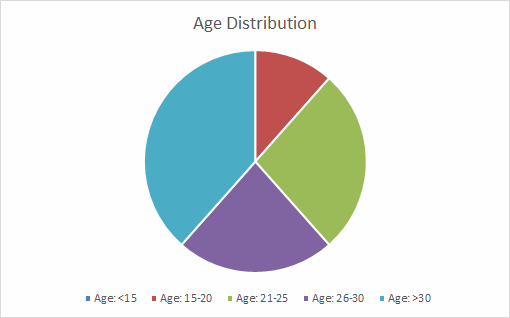
\includegraphics[scale=0.5]{AgePie.png}
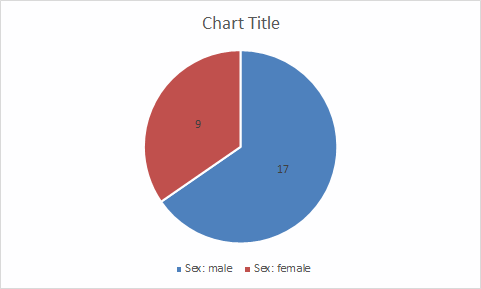
\includegraphics[scale=0.551]{SexPie.png}\\ 
\centering
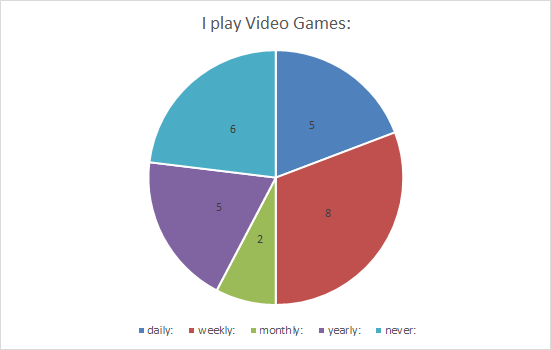
\includegraphics[scale=0.6]{IPlayPie.png}



\section{Feedback}
\raggedright
The feedback was generally positive. We will list the most prominent feedbacks we received. All those feedbacks were independently received multiple times. This Chapter elaborates the feedback for the following aspects of our game: Controls, Sounds, Graphics, Gameplay.

	\subsection{Controls}
	
\begin{enumerate}
\item The way the human player is steering his character seems to be too difficult for inexperienced gamers. They would prefer to control the movement and the rotation of the character with the same joystick. The experienced players on the other hand really appreciate this flexibility. 
\item We have asked the subjects beforehand how they would map the buttons to the different activities. For most mappings they were agreeing with our implementation.
\end{enumerate}	
	
	\subsection{Sounds}
	
	\begin{enumerate}
\item It is naturally a hot topic we are picking up. We tried to only use soft violence (shooting people does not hurt them but solely disperse the group). Nevertheless, the sounds and graphics still seemed to be too violent in the opinion of some of our participants.
\item The sound cues that we included for praying and wonder creation were not registered by the participants. This was due to the shooting sound or the participants yelling being too loud.
\end{enumerate}
	\subsection{Graphics}
	
	\begin{enumerate}
\item Most people enjoyed the obstacles on the map and used them to hide from other players. We got the feedback that a randomly generated map would be nice. Furthermore, they would approve if the map contained more obstacles. Most people enjoyed looking for computer players, which were sometimes hidden behind trees or houses.
\item Some people found the houses to be confusing, as they did not know whether they can be used for anything in the game.
\item Many testers stated that they would like to have visually more separated shots, most would like more flying crosses and Erlenmeyer flasks than the actual energy balls.
\item Darwinists seem to appear to be rendered not as bright as our Religionists which seems to be disturbing for some player.
\item Most of the testers would like to have a symbol or something similar indicating if a praying/studying cycle is creating the wonder and also how fast.
\item In the beginning most people were confused by the amount of characters on the screen and couldn't immediately find their character. Therefore, they suggested to wait a few seconds before the game starts so that one can get an overview of the starting situation. Also they would like to have the colored marker to be filled with the respective color.
\end{enumerate}
	\subsection{Gameplay}
	
	\begin{enumerate}
\item The game is fun. It is not a game people would want to play for a longer period of time, but it is really entertaining when played occasionally. The reason for this might be that they are not challenged enough after some time. This problem is alleviated when people are playing in multi-player mode.
\item Many participants did not make use of the feature to keep the wonder without activating it, and activated the wonder as soon as the wonder bar was full. However, most participants still believe it is an important feature to keep.
\item A lot of testers stated that shooting does not affect the game as much as it should. Most people liked the idea if each character would have a life bar which decreases if the character gets shot and if the life bar is at 0 the character would convert to the other team.
\item If one player casts the, he is too strong because he is invincible. To have a chance to prevent getting converted most testers would like to be able to shoot the player with the wonder, but he should only be affected in X and Y direction so that he can still run with the wonder but gets pushed a little bit into the direction of the shot.
\item Nearly all testers stated that they would like if a player is converted that he can take control over a NPC and not gets converted to the other team. This is the case because people like to identify themselves with a team.
\item Some participants did not use the wonder creation cooldown. They simply prayed/studied until they were shot and flung away.
\end{enumerate}

\section{Alteration Considerations}
The following is a list of things we consider changing, based on the feedback from the testing sessions. The list is not yet prioritized.

\begin{itemize}
	\item \textbf{Sound Leveling:} Shooting and background music must be dimmed. Visual cue for wonder creation must be increased.
		\item \textbf{Wonder Creation Cooldown:} Must be shorter
	\item \textbf{Explosion Force:}  Use less upwards force and balance out the force with the horizontal distanced covered.
	\item \textbf{Shooting:} Use the trigger button (R2) to trigger the shooting action
	\item \textbf{Movement and Look around:} Offer the option to play with combined movement and look around for players that prefer to control their character in such a way.
	\item \textbf{Landscape modification:} Add more obstacles for the players to interact with.
	\item \textbf{Wonder Creation:} Must be indicated better using visual and (hearable) audio cues.
	\item \textbf{Conversion:} After being converted, control an NPC from the same team.
	\item \textbf{Wonder Creation Hit:} Create a wonder penalty when being hit while praying/studying
	\item \textbf{Interface:} Add icons or text to indicate which bar stands for what
	\item \textbf{Create/Cast mapping:} Use the same button type for wonder creation and casting.
	\item \textbf{Wonder Possession:} Use different visual representation than a red disc as a wonder possession representation.
	\item \textbf{Mini Map:} Add a mini map or any indicator to find remote praying/studying groups.
	\item \textbf{Add Running Mode:} Add a running mode where the player can neither shoot nor pray.
	\item \textbf{Outline begind Trees/Houses} Add outline of player when he is behind a tree/house.
\end{itemize}

\section{Appendix: Questionnaire}
We appended the entire questionnaire here.
\label{sec:questionnaire}
\includepdf[pages={2,3,4,5,6}]{../Questionnaire/Questionnaire.pdf}



\end{document}
